\section{Функции для метода конечных элементов}

\subsection{Функции конуса в шаре}

Пусть дана функция следующего вида:
\[
	\varphi(\vec{r}_0, \vec{r}, R) = \begin{cases}
	1 - \frac{\rho}{R}, & \rho < R \\
	0, & \rho \geq R
	\end{cases}
\]
Здесь $\rho = |\vec{r} - \vec{r}_0|$ -- расстояние от текущей точки до $\vec{r}_0$. Для применения в методе конечных элементов необходимо найти интегралы вида:
\[
	I = \int \varphi(\vec{r}_1, \vec{r}, R_1) \varphi(\vec{r}_2, \vec{r}, R_2) dV
\]
Рисунок

\begin{center}
	\begin{tikzpicture}
	\pgfmathsetmacro\rf{2};
	\pgfmathsetmacro\rs{3};
	\pgfmathsetmacro\a {4};
	\pgfmathsetmacro\rh{1.5};
	\pgfmathsetmacro\th{20};
	\pgfmathsetmacro\tmax{acos((\rh*\rh + \a*\a - \rs*\rs)/2/\a/\rh)};
	
	\coordinate (Of) at (0, 0);
	\coordinate (Os) at (\a, 0);
	\coordinate (Rf) at ({\rf*cos(120)}, {-\rf*sin(120)});
	\coordinate (Rs) at ({\rs*cos(120)}, {-\rs*sin(120)});
	\coordinate (Ai) at ({\rh*cos(\tmax)}, {-\rh*sin(\tmax)});
	\coordinate (Ae) at ({\rh*cos(\tmax)}, {\rh*sin(\tmax)});
	\coordinate (Al) at ({\a*cos(\tmax)}, {\a*sin(\tmax)});
	\coordinate (C) at ({\rh*cos(\th)}, {\rh*sin(\th)});
	\coordinate (Cl) at ({\a*cos(\th)}, {\a*sin(\th)});
	\coordinate (angnb) at ({0.8*\a*cos(\th)}, {0.8*\a*sin(\th)});
	\coordinate (angmb) at ({0.3*\rh*cos(-30)}, {0.3*\rh*sin(-30)});
	\coordinate (angme) at ({0.3*\rh*cos(\tmax)}, {0.3*\rh*sin(\tmax)});
	
 	\draw[name path=circle1,black,very thick] (Of) node[left]{$O_1$} circle(\rf) circle(2 pt);
	\draw[name path=circle2,black,very thick] (Os) node[right]{$O_2$} circle(\rs) circle(2 pt);
	\draw[name path=arc1,black,thick] (Ai) arc(-\tmax:\tmax:\rh);
	\draw[thick,dashed] (Of) -- (Os);
	\draw[thick,dashed] (Of) -- (Ae) node[above, midway]{$\rho_1$};
	\draw[thick] (Of) -- (Cl);
	\draw[thick] (C) -- (Os) node[above, midway]{$\rho_2$}; 
	\draw[thick, dashed] (angnb) arc(\th:0:{0.8*\a}) node[right, midway]{$\theta$}; 
	\draw[thick, solid, ->] (angmb) arc(-30:0:{0.3*\rh}) node[below right, midway]{$\theta_m$};
	\draw[thick, solid, <-] (angme) arc(\tmax:\tmax+30:{0.3*\rh});
	\draw[thick, dashed] (Of) -- (Rf) node[right, midway]{$R_1$};
	\draw[thick, dashed] (Os) -- +(Rs) node[right, midway]{$R_2$};
	\end{tikzpicture}
\end{center}

Найдём интеграл $a = O_1O_2$:
\[
\begin{gathered}
	I = \int\limits_{a - R_2}^{R_1} \left(1 - \frac{\rho_1}{R_1}\right) 2\pi \rho_1^2 \int\limits_{0}^{\theta_m(\rho_1)} \left(1 - \frac{\sqrt{\rho_1^2 + a^2 - 2 \rho_1 a \cos \theta}}{R_2}\right) \sin \theta d\theta\, d\rho_1
	= \\ =
	- \int\limits_{a - R_2}^{R_1} \left(1 - \frac{\rho_1}{R_1}\right) 2\pi \rho_1^2 \left(\cos \theta + \frac{\left(\rho_1^2 + a^2 - 2 \rho_1 a \cos \theta\right)^{3/2}}{3a\rho_1R_2}\right) \Bigg|_0^{\theta_m} d\rho_1
	= \\ =
	- \int\limits_{a - R_2}^{R_1} \left(1 - \frac{\rho_1}{R_1}\right) 2\pi \rho_1^2 
	\left(
	\frac{a^2 + \rho_1^2 - R_2^2}{2a\rho_1} - 1 + 
	\frac{R_2^2}{3a\rho_1} -
	\frac{(a - \rho_1)^3}{3a\rho_1R_2}
	\right) d\rho_1
\end{gathered}
\]
Сделаем замену:
\[
	x = \rho_1 + R_2 - a \qquad \rho_1 = x - R_2 + a \qquad a - \rho_1 = R_2 - x
\]
\[
\begin{gathered}
	I = - \frac{2\pi}{R_1 a} \int\limits_{0}^{x_m = R_1 + R_2 - a} (R_1 + R_2 - a - x) (x - R_2 + a) 
	\left(
	\frac{(a - \rho_1)^2 - R_2^2}{2} + 
	\frac{R_2^2}{3} -
	\frac{(R_2 - x)^3}{3R_2}
	\right) dx
	= \\ =
	- \frac{2\pi}{R_1 a} \int\limits_{0}^{x_m} (R_1 + R_2 - a - x) (x - R_2 + a) 
	\left(
	\frac{x^2 - 2 x R_2}{2} + 
	\frac{R_2^2}{3} -
	\frac{R_2^3 - 3 R_2^2 x + 3 R_2 x^2 - x^3}{3R_2}
	\right) dx
	= \\ =
	- \frac{2\pi}{R_1 a} \int\limits_{0}^{x_m} (R_1 + R_2 - a - x) (x - R_2 + a) 
	\left(
	- \frac{x^2}{2} +
	\frac{x^3}{3R_2}
	\right) dx
	= \\ =
	\frac{\pi}{3 R_1 R_2 a} \int\limits_{0}^{x_m} (x_m - x) (x - x_m + R_1) x^2  
	\left(
	3 R_2 - 2 x
	\right) dx
	= \\ =
	\frac{\pi}{3 R_1 R_2 a} \int\limits_{0}^{x_m} (- 3 R_2 x^4 - 3 R_2 x_m^2 x^2 + 6 R_2 x_m x^3 + 3 R_2 R_1 x_m x^2 - 3 R_2 R_1 x^3 + 2 x^5 + 2 x_m^2 x - 4 x_m x^4 - 2 R_1 x_m x^3 + 2 R_1 x^4)  
	dx
	= \\ =
	\frac{\pi}{3 R_1 R_2 a} (- 3 R_2 x_m^5/5 - 3 R_2 x_m^5 / 3  + 6 R_2 x_m^5/4 + 3 R_2 R_1 x_m^4/3 - 3 R_2 R_1 x_m^4/4 + 2 x_m^6/6 + 2 x_m^6/4 - 4 x_m^6/5 - 2 R_1 x_m^5/4 + 2 R_1 x_m^5/5)
	= \\ =
	\frac{\pi}{3 R_1 R_2 a} (- R_2 x_m^5/10 + R_2 R_1 x_m^4/4 + x_m^6 / 30 - R_1 x_m^5/10)
	= \\ =
	\frac{\pi}{3 R_1 R_2 a} (- (R_2 + R_1) x_m^5/10 + R_2 R_1 x_m^4/4 + x_m^6 / 30)	
	= \\ =
	\frac{\pi}{180 R_1 R_2 a} (- 6 (R_2 + R_1) x_m + 15 R_2 R_1 + 2 x_m^2) x_m^4
	= \\ =
	\frac{\pi}{180 R_1 R_2 a} (- 6 (R_2 + R_1)^2 + 6 (R_2 + R_1) a + 15 R_2 R_1 + 2 (R_2 + R_1)^2 - 4 (R_2 + R_1) a + 2 a^2) x_m^4
	= \\ =
	\frac{\pi}{180 R_1 R_2 a} (- 4 R_2^2 - 4 R_1^2 + 2 (R_2 + R_1) a + 7 R_2 R_1 + 2 a^2) x_m^4
\end{gathered}
\]

Всё блажь! Не сходится ничего. Надо три варианта рассматривать, убиться можно!

\subsection{Пирамиды в тетраэдре}

Пусть функция равна единице на вершине и нулю на противоположной вершине грани (плоскости). Её можно представить в виде:
\[
	u_1 = 1 - \frac{h_1}{H_1} = 1 - \frac{V_1}{V} = 1 - \frac{\begin{vmatrix}
		x   & y   & z   & 1 \\
		x_2 & y_2 & z_2 & 1 \\
		x_3 & y_3 & z_3 & 1 \\
		x_4 & y_4 & z_4 & 1
		\end{vmatrix}}{\begin{vmatrix}
		x_1 & y_1 & z_1 & 1 \\
		x_2 & y_2 & z_2 & 1 \\
		x_3 & y_3 & z_3 & 1 \\
		x_4 & y_4 & z_4 & 1
		\end{vmatrix}}
\]
Найдём интегралы вида:
\[
	\int\limits_V u_1 u_2 dV \quad \int\limits_V u_1 dV
\]
Посмотрим на рисунок:
\begin{center}
	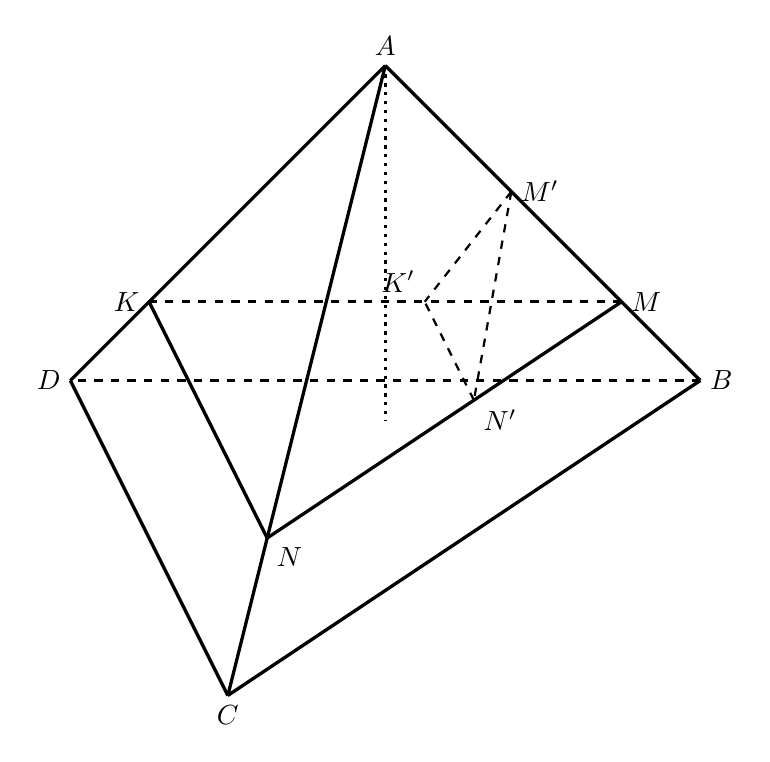
\begin{tikzpicture}
	\coordinate (A) at (4, 4);
	\coordinate (B) at (8, 0);
	\coordinate (C) at (2,-4);
	\coordinate (D) at (0, 0);
	\coordinate (M) at (7, 1);
	\coordinate (N) at (2.5,-2);
	\coordinate (K) at (1, 1);
	\coordinate (H) at (4,-0.5);
	\coordinate (Ms) at (5.6, 2.4);
	\coordinate (Ns) at (5.125, -0.25);
	\coordinate (Ks) at (4.5, 1);
	
	\draw (A) node[above]{$A$};
	\draw (B) node[right]{$B$};
	\draw (C) node[below]{$C$};
	\draw (D) node[left]{$D$};
	\draw (M) node[right]{$M$};
	\draw (N) node[below right]{$N$};
	\draw (K) node[left]{$K$};
	\draw (Ms) node[right]{$M'$};
	\draw (Ns) node[below right]{$N'$};
	\draw (Ks) node[above left]{$K'$};
	
	\draw[solid, very thick]  (A) -- (B);
	\draw[solid, very thick]  (A) -- (C);
	\draw[solid, very thick]  (A) -- (D);
	\draw[solid, very thick]  (B) -- (C);
	\draw[dashed, very thick] (B) -- (D);
	\draw[solid, very thick]  (C) -- (D);
	
	\draw[solid, very thick]  (M) -- (N);
	\draw[dashed, very thick] (M) -- (K);
	\draw[solid, very thick]  (N) -- (K);
	
	\draw[dashed, thick]  (Ms) -- (Ns);
	\draw[dashed, thick]  (Ms) -- (Ks);
	\draw[dashed, thick]  (Ns) -- (Ks);
	
	\draw[dotted, very thick] (A) -- (H);
	\end{tikzpicture}
\end{center}

Обозначим $x = MK'$, $l = K'N'$, $a = MK$, $\angle CDB = \alpha$, расстояние от плоскости $MNK$ до плоскости $BCD$ -- $h_1$, расстояние от точки $A$ до плоскости $BCD$ -- $H_1$, расстояние от точки $M$ до плоскости $ACD$ -- $h_t$, расстояние от прямой $K'N'$ до плоскости $ACD$ -- $h_2$, расстояние от точки $B$ до плоскости $ACD$ -- $H_2$. Воспользуемся подобием треугольников:
\[
	\frac{l}{CD} = \frac{x}{BD}
\]
\[
	\frac{a}{BD} = \frac{H_1 - h_1}{H_1} = 1 - \frac{h_1}{H_1}
\]
\[
	\frac{h_t}{H_2} = \frac{a}{BD} = 1 - \frac{h_1}{H_1}
\]
\[
	\frac{x}{a} = \frac{h_t - h_2}{h_t} = 1 - \frac{h_2}{h_t} =
	1 - \frac{h_2}{H_2\left(1 - \frac{h_1}{H_1}\right)}
\]
\[
	1 - \frac{h_2}{H_2} = \frac{x}{a} \left(1 - \frac{h_1}{H_1}\right) + \frac{h_1}{H_1}
\]
\[
	\boxed{
	\begin{gathered}
	\int\limits_V u_1 u_2 dV = 
	\int\limits_{0}^{H_1} \left(1 - \frac{h_1}{H_1}\right) \int\limits_{0}^{a}  \left(\frac{x}{a} \left(1 - \frac{h_1}{H_1}\right) + \frac{h_1}{H_1}\right) l \sin \alpha \, dx \, dh_1 
	= \\ =
	\frac{CD\cdot H_1 \sin \alpha}{BD}
	\int\limits_{0}^{1} (1 - y) \int\limits_{0}^{1}  \left(z \left(1 - y\right) + y\right) z a^2 \, dz \, dy
	= \\ =
	BD\cdot CD\cdot H_1 \sin \alpha
	\int\limits_{0}^{1} (1 - y)^3 \int\limits_{0}^{1}  \left(z \left(1 - y\right) + y\right) z \, dz \, dy
	= 
	6 V
	\int\limits_{0}^{1} (1 - y)^3 \left(\frac{1 - y}{3} + \frac{y}{2}\right) dy
	= \\ =
	6 V
	\int\limits_{0}^{1} p^3 \left(- \frac{p}{6} + \frac{1}{2}\right) dp
	=
	6 V \left(\frac{1}{8} - \frac{1}{30}\right) = 6 V \frac{15 - 4}{120} = \frac{11}{20} V
	\end{gathered}
	}
\]
\[
\boxed{
	\begin{gathered}
	\int\limits_V u_1 dV = 
	\int\limits_{0}^{H_1} \left(1 - \frac{h_1}{H_1}\right) \int\limits_{0}^{a}  l \sin \alpha \, dx \, dh_1 
	=
	\frac{CD\cdot H_1 \sin \alpha}{BD}
	\int\limits_{0}^{1} (1 - y) \int\limits_{0}^{1} z a^2 \, dz \, dy
	= \\ =
	6 V
	\int\limits_{0}^{1} (1 - y)^3 \int\limits_{0}^{1} z \, dz \, dy
	= 
	3 V
	\int\limits_{0}^{1} (1 - y)^3 dy
	=
	\frac{3}{4} V
	\end{gathered}
}
\]
Порой требуется искать производные и интегралы от производных от функций такого вида. Найдём одну производную:
\[
	\frac{\partial u}{\partial x} = - \frac{1}{V} \frac{\partial V_1}{\partial x}
	=
	- \frac{\begin{vmatrix}
	1   & 0   & 0   & 0 \\
	x_2 & y_2 & z_2 & 1 \\
	x_3 & y_3 & z_3 & 1 \\
	x_4 & y_4 & z_4 & 1
	\end{vmatrix}}{\begin{vmatrix}
	x_1 & y_1 & z_1 & 1 \\
	x_2 & y_2 & z_2 & 1 \\
	x_3 & y_3 & z_3 & 1 \\
	x_4 & y_4 & z_4 & 1
	\end{vmatrix}}
	=
	- \frac{S_{\text{пр. 1 грани }x}}{V}
\]